\documentclass{standalone}
\usepackage{tikz}
\usepackage{lmodern}

\begin{document}
	
	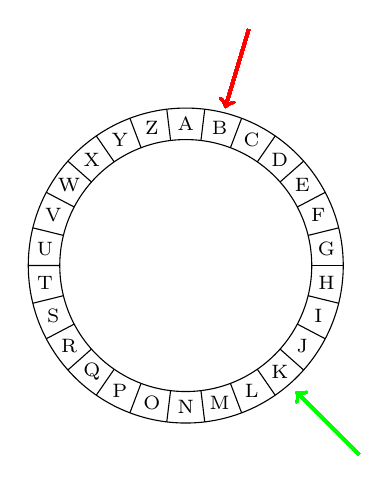
\begin{tikzpicture}
		\def\alphabet{{"A","B","C","D","E","F","G","H","I","J","K","L","M","N","O","P","Q","R","S","T","U","V","W","X","Y","Z"}}
		
		\draw (0,0) circle(2cm); 
		\draw (0,0) circle(1.6cm); 
		
		\foreach \i [count=\j from 0] in {0,13.846,...,346.154} {
			\draw (\i:1.6cm) -- (\i:2cm);  
			\node at (\i+90+13.846:1.8cm) {\scriptsize \pgfmathparse{\alphabet[25-\j]}\pgfmathresult};  
			\draw[red, very thick, ->] (0.8, 3) -- (0.5,2);
			\draw[green, very thick, ->] (2.2, -2.4) -- (1.4, -1.6);
		}
	\end{tikzpicture}
	
\end{document}
